\section{O problema da tradução entre representações computacionais}

Conforme discutido nos capítulos anteriores, uma mesma lógica computacional pode ser expressa por diferentes representações, como linguagens textuais, fluxogramas, \textit{blueprints} e plataformas \textit{Low-Code} ou \textit{No-Code}, todas capazes de descrever decisões, condições e fluxos de execução.

O problema central abordado por esta pesquisa está no fato de que essas representações são desenvolvidas e utilizadas como ambientes isolados entre si. Cada ferramenta define sua própria sintaxe, sua própria semântica e seu próprio modo de construir a lógica, sem mecanismos que permitam transitar de uma representação para outra. Na prática, uma lógica construída em um ambiente não pode ser reaproveitada em outro: para migrar de uma representação textual para uma visual, ou vice-versa, é necessário reconstruí-la manualmente desde o início.

Essa ausência de comunicação entre representações gera retrabalho, dificulta a colaboração entre perfis técnicos distintos e impede que o conhecimento expresso em uma forma seja transferido diretamente para outra. Diante disso, coloca-se a questão que motiva esta proposta: seria possível identificar uma estrutura lógica comum a essas representações, capaz de servir de base para converter uma na outra sem perda de significado computacional? É essa questão que as seções seguintes buscam responder.

\section{Lógica computacional como estrutura intermediária}

A resposta que esta pesquisa propõe para a questão levantada anteriormente é que essa estrutura comum é a própria lógica computacional, compreendida de forma independente da representação que a expressa. Embora linguagens de programação, fluxogramas, \textit{blueprints} e plataformas \textit{Low-Code} ou \textit{No-Code} apresentem diferenças visuais e sintáticas, todas descrevem os mesmos elementos fundamentais: decisões, condições, operações, eventos e sequências de execução.

A proposta é tratar esses elementos fundamentais como uma camada situada entre a lógica e suas diferentes formas de representação. Nessa camada, a lógica deixa de estar presa à sintaxe de uma linguagem ou ao formato gráfico de uma ferramenta e passa a ser descrita de forma abstrata: uma condição é apenas uma condição, com seus possíveis desfechos, e uma sequência de operações é apenas uma ordem de execução, sem depender de como cada ambiente a desenha ou escreve. É essa descrição abstrata, despida da forma, que constitui a estrutura lógica intermediária.

Essa ideia apoia-se no conceito de abstração discutido no Capítulo 2 \cite{abelson1996}. Da mesma forma que uma linguagem de alto nível oculta detalhes de implementação sem alterar o comportamento do programa, a estrutura lógica intermediária oculta as particularidades de cada representação, preservando apenas aquilo que define o comportamento computacional. Assim, fluxogramas, \textit{blueprints} e código textual passam a ser vistos como diferentes projeções de uma mesma estrutura.

Compreender a lógica dessa forma é o que torna a tradução entre representações conceitualmente possível. Se duas representações podem ser reduzidas à mesma estrutura intermediária, é possível interpretar uma delas, identificar sua estrutura lógica e, a partir dela, gerar a outra, sem perda do comportamento originalmente definido.

Um exemplo simples ilustra esse princípio. A decisão de verificar se uma idade é maior ou igual a 18 pode ser escrita em código como uma estrutura \texttt{if/else}, desenhada em um fluxograma como um losango de decisão com dois caminhos, ou montada em um \textit{blueprint} como um nó de comparação com duas saídas. As três formas têm aparência completamente diferente, mas descrevem a mesma estrutura intermediária: uma condição com dois desfechos possíveis. O que muda é a forma; a lógica permanece a mesma.

A Figura \ref{fig:estrutura_intermediaria} resume essa ideia, posicionando a lógica computacional como substrato comum a partir do qual as diferentes representações podem ser interpretadas.
\begin{figure}[H]
    \centering
    \caption{Representação conceitual da lógica computacional como estrutura intermediária entre diferentes formas de representação computacional.}
    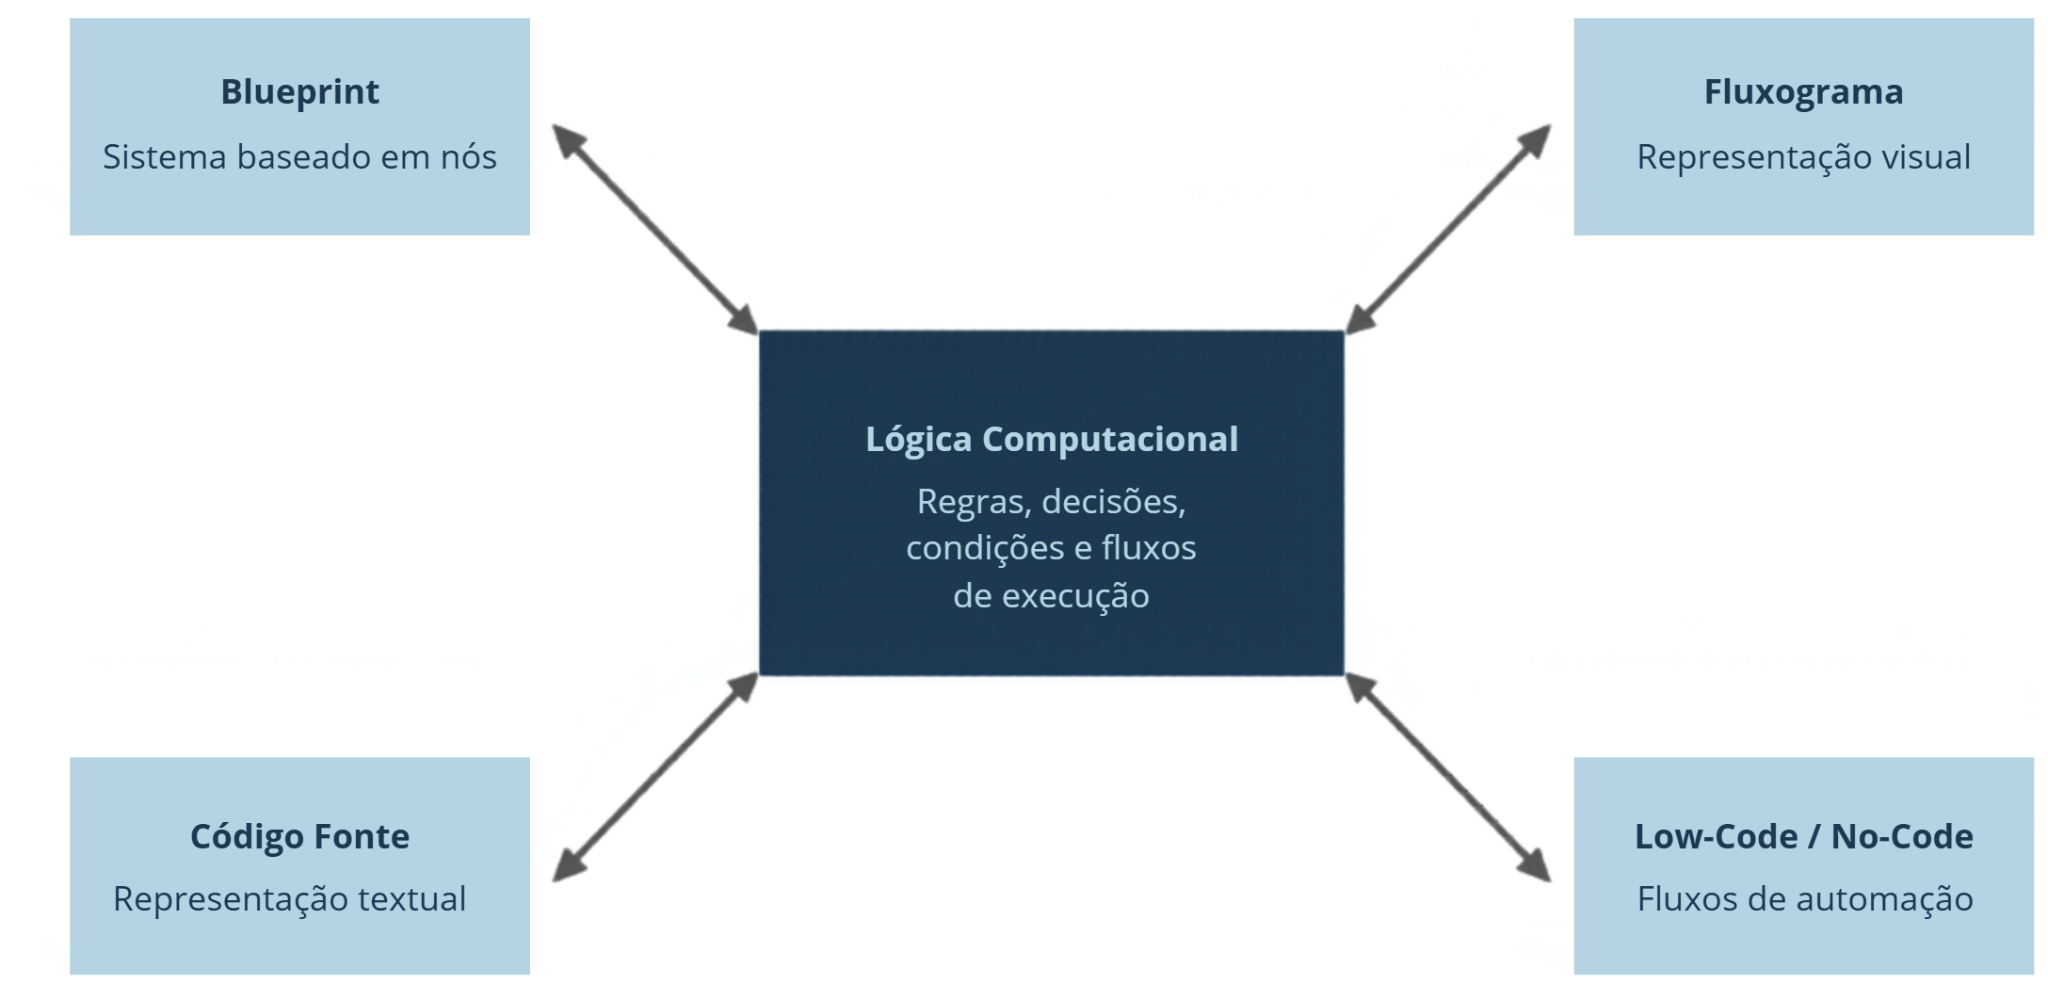
\includegraphics[width=\textwidth]{images/estrutura_intermediaria.png}
    \legend{Fonte: elaboração do autor com base em \citeonline{abelson1996} e \citeonline{myers1990}.}
    \label{fig:estrutura_intermediaria}
\end{figure}

\section{Modelo conceitual proposto}

Com base na hipótese desenvolvida na seção anterior, esta pesquisa propõe um modelo conceitual de conversão organizado em três etapas. Na primeira, uma representação de origem é interpretada, e sua lógica é extraída na forma da estrutura lógica intermediária. Na segunda, essa estrutura mantém a lógica de maneira abstrata, independente de qualquer linguagem ou ferramenta. Na terceira, a partir dessa estrutura, gera-se uma representação de destino, textual ou visual, preservando o comportamento originalmente definido.

O ponto central desse modelo é que a conversão nunca ocorre diretamente de uma representação para outra, mas sempre por meio da estrutura intermediária. Essa escolha não é apenas conceitual: converter cada representação diretamente em todas as demais exigiria um mecanismo específico para cada par de formatos, e a quantidade desses mecanismos cresceria rapidamente a cada nova representação incluída. Ao adotar uma estrutura intermediária comum, basta que cada representação saiba ser interpretada para essa estrutura e gerada a partir dela, reduzindo o problema a um conjunto menor e reaproveitável de etapas.

Para que isso seja possível, o modelo considera que elementos como condições, operações, eventos e sequências de execução podem ser identificados em qualquer representação e organizados nessa estrutura comum. São esses elementos, e não a aparência de cada ambiente, que o modelo preserva ao longo de todo o processo de conversão.

A Figura \ref{fig:modelo_conceitual} representa esse fluxo, no qual uma representação de origem é interpretada, convertida na estrutura lógica intermediária e, a partir dela, transformada em uma representação de destino.
\begin{figure}[H]
\centering
\caption{Modelo conceitual proposto para conversão entre representações computacionais.}
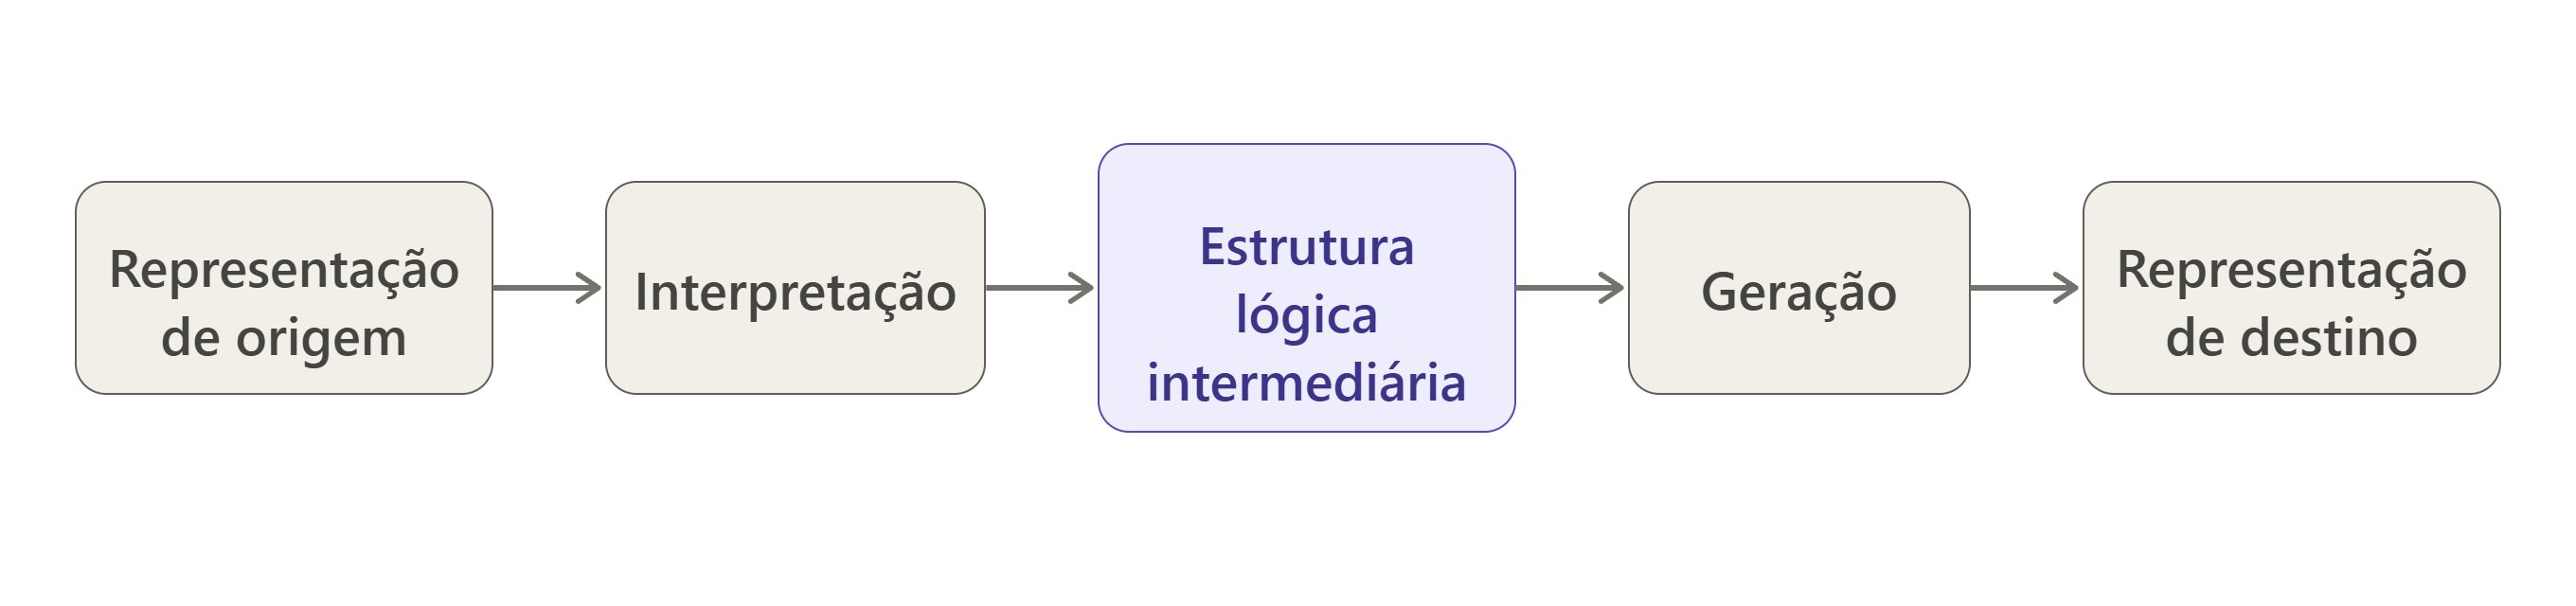
\includegraphics[width=\textwidth]{images/figura6_modelo_conceitual.png}
\legend{Fonte: elaboração do autor.}
\label{fig:modelo_conceitual}
\end{figure}



\section{Cenários de conversão entre representações}

Conforme antecipado na introdução, a inteligência artificial pode atuar como mecanismo de apoio nesse processo de conversão. Em vez de depender de regras fixas definidas manualmente para cada par de representações, um mecanismo assistido por IA poderia identificar a estrutura lógica subjacente a uma representação de origem e reconstruí-la em uma representação de destino. Dessa forma, a IA atuaria como uma camada responsável por interpretar, comparar e gerar representações computacionais, preservando o comportamento lógico originalmente definido.

Nesse contexto, um algoritmo descrito em código-fonte pode ser convertido para um fluxograma, assim como um fluxograma pode ser transformado em uma representação textual equivalente. O mesmo princípio pode ser aplicado a sistemas baseados em nós e plataformas \textit{Low-Code} ou \textit{No-Code}, desde que a lógica computacional subjacente seja preservada durante o processo de conversão. 

A Figura \ref{fig:arquitetura_camada_ia} apresenta a arquitetura conceitual do modelo, destacando o papel da IA como camada mediadora entre as representações e a estrutura lógica subjacente.

\begin{figure}[H]
\centering
\caption{Arquitetura conceitual da camada de IA como elemento mediador entre representações computacionais.}
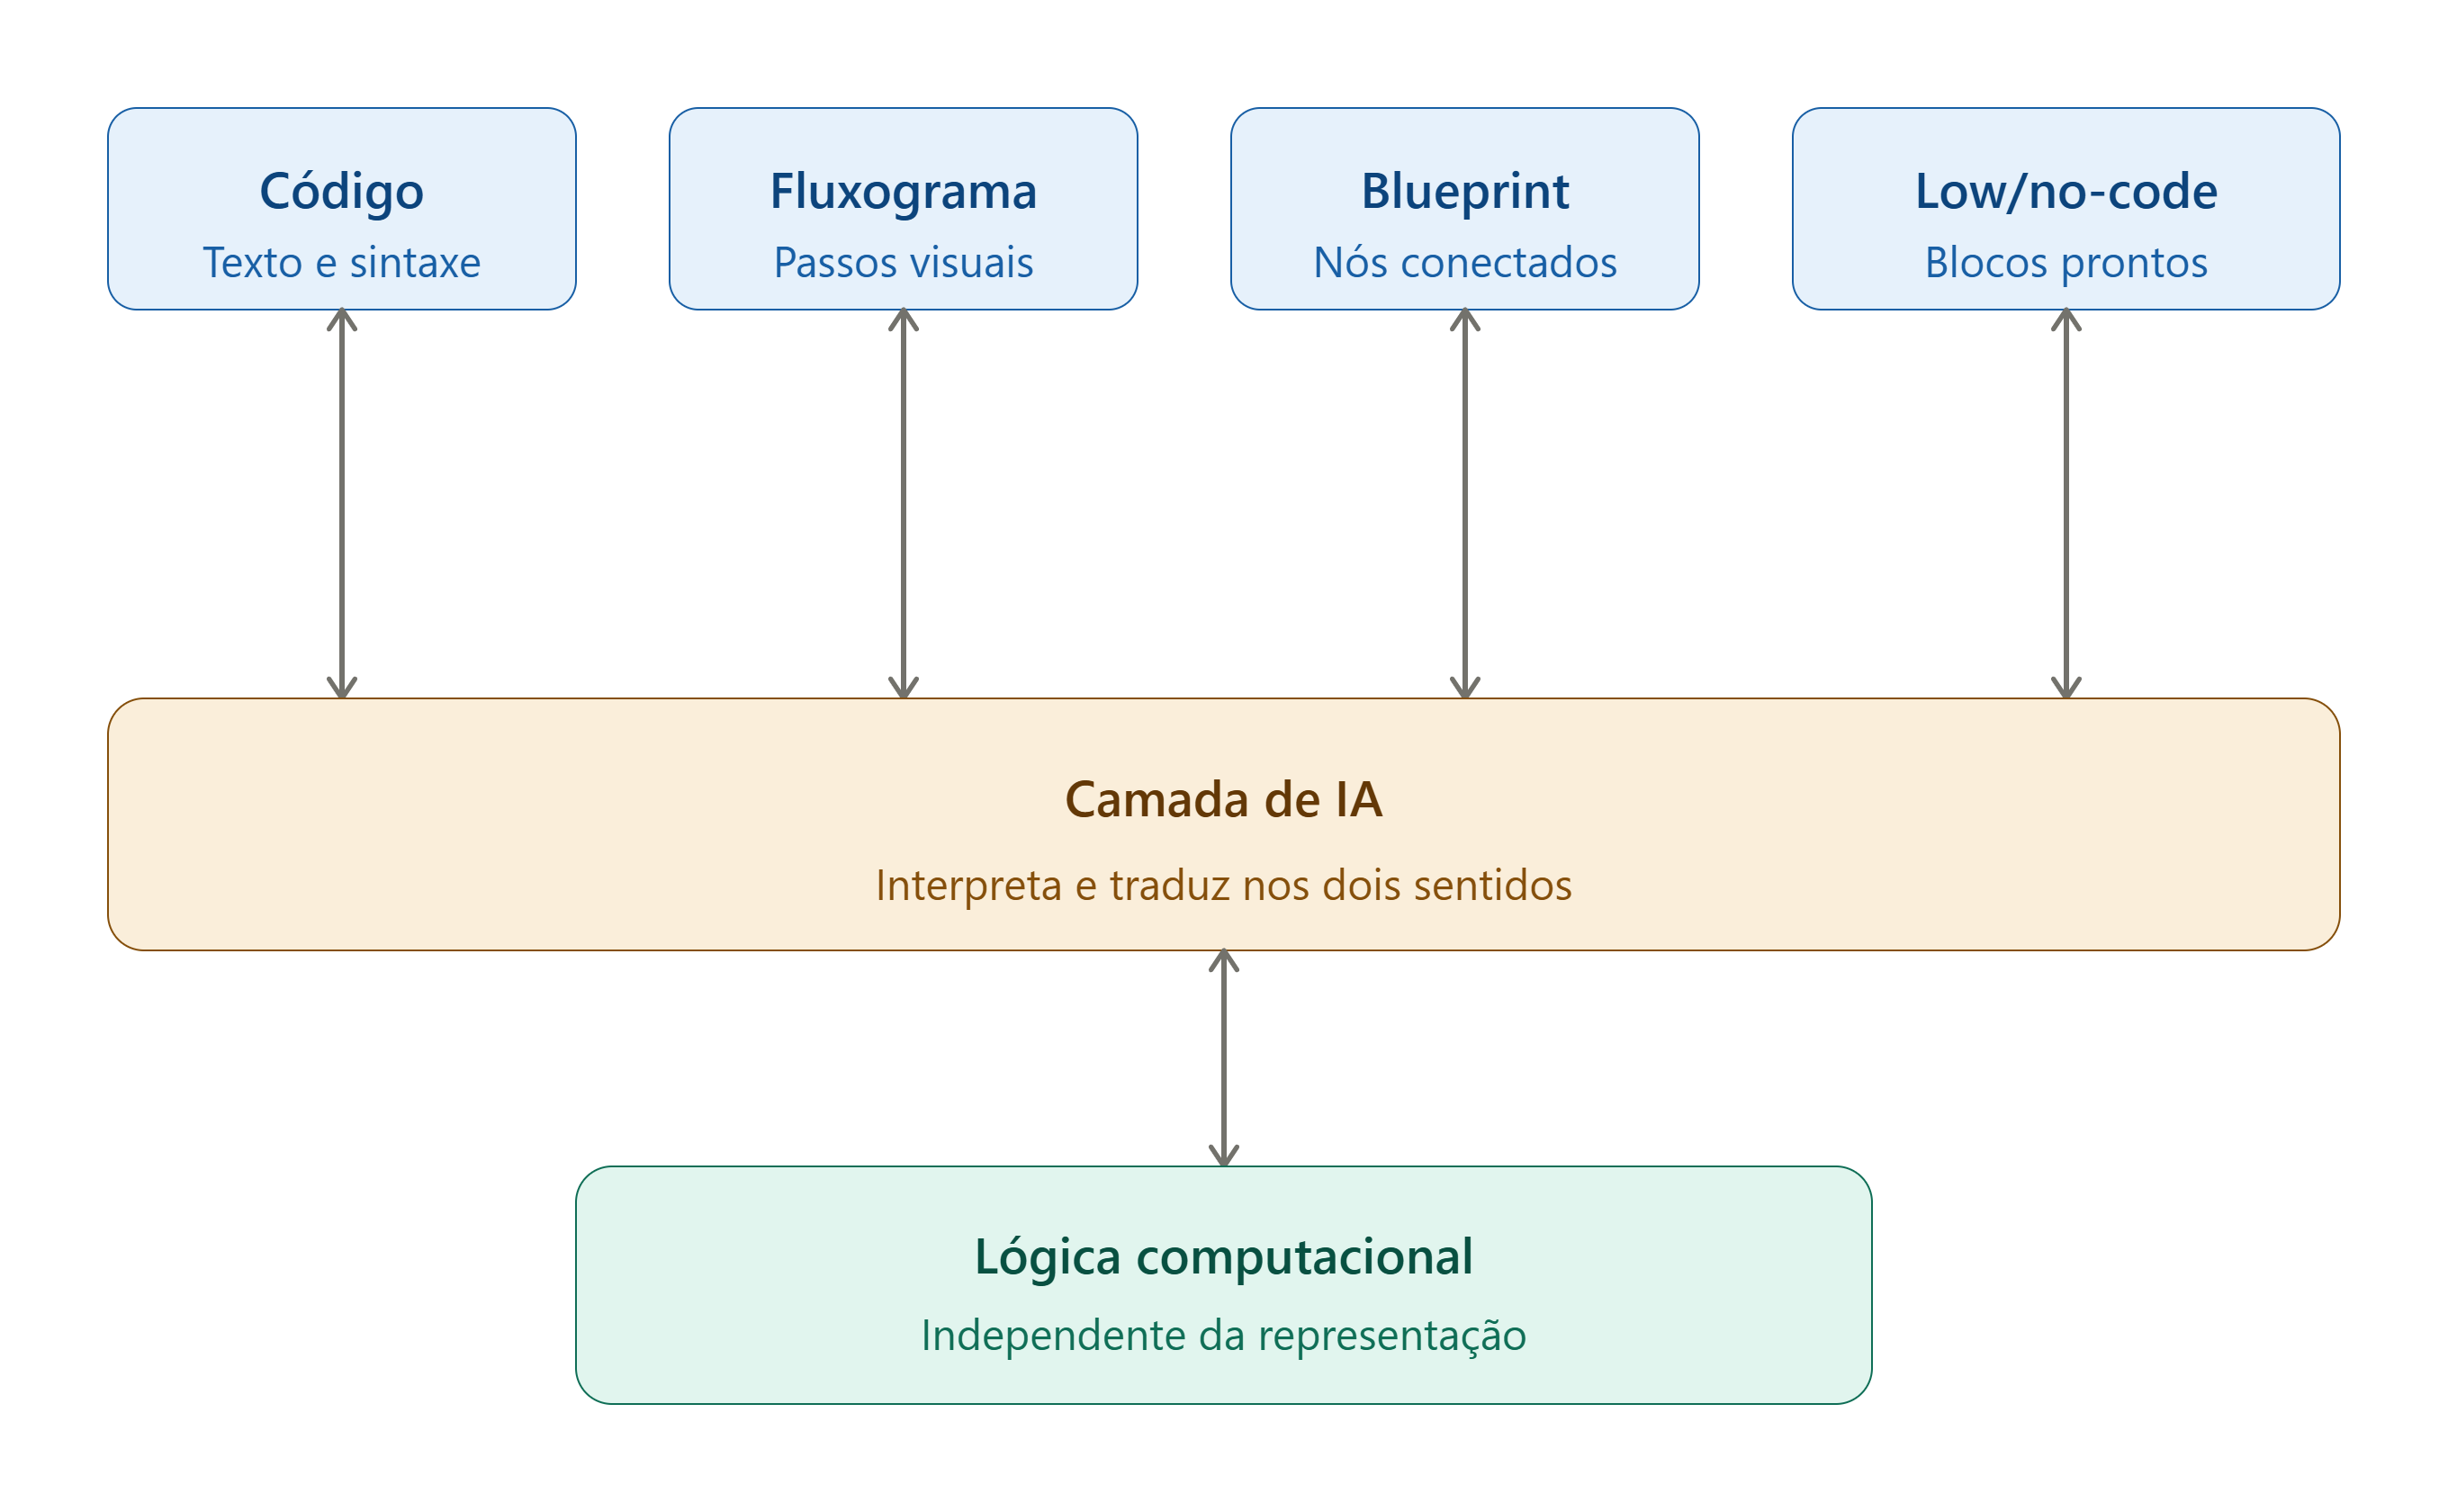
\includegraphics[width=\textwidth]{images/arquitetura_camada_ia.png}
\legend{Fonte: elaboração do autor.}
\label{fig:arquitetura_camada_ia}
\end{figure}

A partir dessa perspectiva, diferentes representações computacionais podem ser compreendidas como manifestações distintas de uma mesma lógica computacional. Dessa forma, a conversão entre código-fonte, fluxogramas, \textit{blueprints} e plataformas \textit{Low-Code} ou \textit{No-Code} \cite{silva2024lowcode} torna-se conceitualmente possível por meio da identificação de uma estrutura lógica intermediária, preservando o significado computacional originalmente definido.

\section{Limitações da proposta}

Esta pesquisa tem caráter conceitual e exploratório, conforme definido em sua metodologia. Por essa razão, não contempla o desenvolvimento de um sistema funcional de tradução nem a validação experimental do modelo: a precisão, a viabilidade e o desempenho de um mecanismo de conversão constituem uma etapa posterior, que pressupõe a base conceitual aqui estabelecida.

No plano técnico, há a diversidade entre os ambientes de desenvolvimento. Embora diferentes representações compartilhem princípios lógicos semelhantes, cada ferramenta possui sua própria sintaxe, semântica e forma de execução, e determinados recursos de uma representação podem não ter equivalente direto em outra. Esses casos delimitam até onde a tradução pode ser automática, indicando pontos em que mecanismos de adaptação seriam necessários.

O modelo concentra-se ainda na lógica interna de um algoritmo: suas decisões, condições e fluxos de execução. Aspectos que extrapolam essa lógica, como dependências de serviços externos ou a coordenação entre componentes distribuídos, não fazem parte do escopo desta proposta. Delimitar a análise à estrutura lógica é uma escolha deliberada, que permite isolar o problema central da pesquisa.

Apesar dessas limitações, a proposta oferece uma contribuição própria: um modelo conceitual que trata a lógica computacional como elemento separável de sua forma de representação, fornecendo uma base teórica para a tradução entre representações distintas. A partir dessa base, a implementação e a validação prática apresentam-se como continuidade natural desta pesquisa.